\documentclass[12pt]{article}
\usepackage{amsfonts, epsfig}
\usepackage[authoryear]{natbib}
\usepackage{graphicx}
\usepackage{fancyhdr}
\pagestyle{fancy}
\lfoot{\texttt{comsm0075.github.io}}
\lhead{IP\&B - 1\_the\_Bayesian\_brain - Conor}
\rhead{\thepage}
\cfoot{}
\begin{document}

\section*{Sensory processing and probabalistic codes.}

In this section we will begin to explore the idea that the brain
performs Bayesian inference on data. However, we will begin by looking at a cartoon \texttt{https://xkcd.com/1132/}

\begin{center}
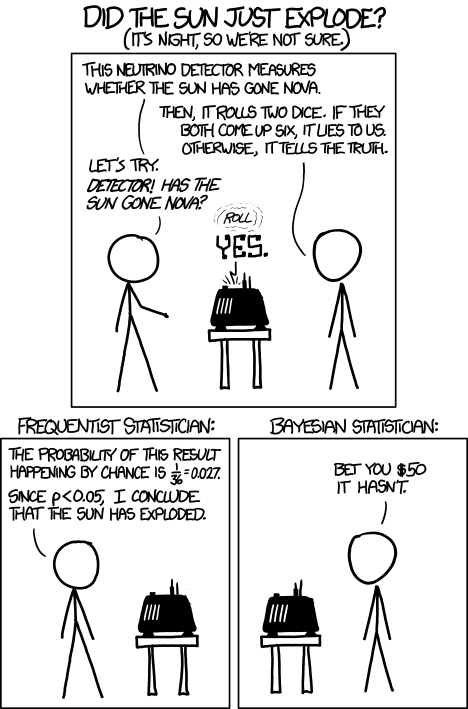
\includegraphics[width=7.5cm]{frequentists_vs_bayesians.png}
\end{center}

So; will the Bayesian win his or her bet? I will start by annoyingly
over explaining the joke; the frequentist knows the detector only lies
one time in 36, so he or she assumes that the detector isn't
lying. However, the Bayesian takes into account the unlikeness of
the detector's statement when estimating the probability its
statement is true. In other words, the frequentist is only paying
attention to the evidence, the Bayesian also considers how likely the
situation the evidence points to is. Randall Munroe's point is that
the sort of mistake the frequentist is making is actually made very
often, but by illustrating it in this extreme example, the sun is very
unlikely to explode, he shows how ridiculous a mistake it is. 

Recall Bayes's rule; if $X$ and $Y$ are two random variables then
\begin{equation}
P(X|Y)=\frac{P(Y|X)P(X)}{P(Y)}
\end{equation}
In this case lets use $D$ to denote the random variable, with $D=w$
denoting a warning from the detector; let $S$ be the state of the sun,
with $S=n$ for the sun exploding and $S=f$ for the sun staying fine,
that is, not exploding. Now the cartoon tells us that
\begin{equation}
P(D=w|S=n)=\frac{35}{36}
\end{equation}
and since this is close to one, the silly frequentist assumes the sun
has exploded. Let's assume the probability the sun has exploded is one
in a million; it is actually much less than that, so
$P(S=n)=10^{-6}$. Now, what we want to know is $P(S=f|D=w)$, the probability the sun hasn't exploded given that detector has warned that it has, now
\begin{equation}
P(S=f|D=w)=\frac{P(D=w|S=f)P(S=f)}{P(W)}
\end{equation}
The numerator we can calculated easily:
\begin{equation}
P(D=w|S=f)P(S=f)=\frac{1}{36}(1-10^{-6})
\end{equation}
because the detector will only say the sun is exploding when it isn't when two dice show sixes, that is, one time in 36. The denominator requires marginalizing:
\begin{equation}
P(D=w)=P(D=w,S=n)+P(D=w,S=f)
\end{equation}
and, using $P(X,Y)=P(X|Y)P(Y)$ this gives
\begin{eqnarray}
P(D=w) &=& P(D=w|S=n)P(S=n)+P(D=w|S=f)P(S=f)\cr
&&=\frac{35}{36}10^{-6}+\frac{1}{36}(1-10^{-6})
\end{eqnarray}
Substituting all this in to Bayes's rule gives:
\begin{equation}
P(S=f|D=w)\approx 0.999965
\end{equation}

The point of this section is that the brain is more like the Bayesian than the frequentist!

\subsection*{Bayesians versus frequentists}

Commenting on the response to his cartoon, Randall Monroe says this\footnote{see http://www.explainxkcd.com/wiki/index.php/1132:\_Frequentists\_vs.\_Bayesians}

\begin{quote}
Hey! I was kinda blindsided by the response to this comic.

I'm in the middle of reading a series of books about forecasting
errors (including Nate Silver's book, which I really enjoyed), and
again and again kept hitting examples of mistakes caused by blind
application of the textbook confidence interval approach.

Someone asked me to explain it in simple terms, but I realized that in
the common examples used to illustrate this sort of error, like the
cancer screening/drug test false positive ones, the correct result is
surprising or unintuitive. So I came up with the sun-explosion
example, to illustrate a case where na\"{i}ve application of that
significance test can give a result that's obviously nonsense.

I seem to have stepped on a hornet's nest, though, by adding
\lq{}Frequentist\rq{} and \lq{}Bayesian\rq{} titles to the
panels. This came as a surprise to me, in part because I actually
added them as an afterthought, along with the final punchline. (I
originally had the guy on the right making some other cross-panel
comment, but I thought the \lq{}bet\rq{} thing was cuter.)

The truth is, I genuinely didn't realize Frequentists and Bayesians
were actual camps of people - all of whom are now emailing me. I thought
they were loosely-applied labels - perhaps just labels appropriated by
the books I had happened to read recently for the standard textbook
approach we learned in science class versus an approach which more
carefully incorporates the ideas of prior probabilities.

I meant this as a jab at the kind of shoddy misapplications of
statistics I keep running into in things like cancer screening (which
is an emotionally wrenching subject full of poorly-applied
probability) and political forecasting. I wasn't intending to
characterize the merits of the two sides of what turns out to be a
much more involved and ongoing academic debate than I realized.

A sincere thank you for the gentle corrections; I've taken them to
heart, and you can be confident I will avoid such mischaracterizations
in the future!

At least, 95.45\% confident.
\end{quote}

Since the rules of probability are fixed it seems odd that there are
different \lq{}camps\rq{}; but there are certainly two different
approaches to statistics described by frequentist and Bayesian. The
difference comes down to different interpretations of what we are
talking about when we talk about randomness. For a frequentist a
random event is truly random, like putting a Geiger counter beside a
radioactive source and an observation is a deterministic process which
definitively checks whether how many decays a Geiger counter has
counted. 

For a Bayesian randomness is a representation of our ignorance. An
example might be a weather prediction; when I am intending to cycle to
Bath I check the weather on my phone and it might say that there is a
27\% chance of rain at 5pm. This doesn't mean that there is a random
process that 27\% of the time will cause rain and the other 73\% cause
not rain. It means that according to the measurements made by the
weather service the state of the weather is such that, based on
previous experience, it will rain 27\% of the time. This situation can
change, it might start raining now and this new evidence would make it
more likely it will rain at 5pm; the situation would also change if
the weather service decided helping me avoid rain was a priority so
more weather detectors and satellite imaging resources should be
directed at predicting rain between Bristol and Bath; this would
change the predictions without changing the actual chance of rain.

\begin{figure}[htb]
\begin{center}
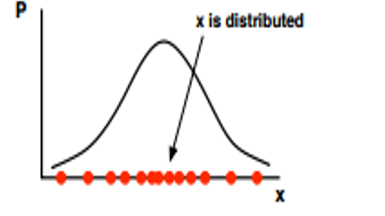
\includegraphics[width=5.5cm]{fig_freq.png}
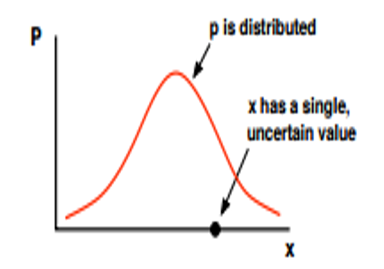
\includegraphics[width=5cm]{fig_bayes.png}
\end{center}
\caption{Frequentist versus Bayesian. The left picture illustrates a
  frequentist interpretation, the right, a Bayesian one. [Pictures
    from Rosalyn Moran]\label{fig_freq_v_bayes}}
\end{figure}


In an extreme description, in the frequentist picture a random
variable will have many values, they will be different because the
process that produces the outcome is random. In the Bayesian picture,
there is just one thing being observed; the state of some variable,
the probability distribution models our knowledge of its value. This
situation is illustrated in Fig.~\ref{fig_freq_v_bayes}. The two
pictures, of course, intersect, for example, in the Bayesian picture
our partial knowledge of variable is sometimes attributed to noise in
the sensors we use to measure it, this noise is a random event in the
frequentist sense.


In this way there isn't an argument between frequentists and Bayesians
about the laws of probability; rather, frequentist and Bayesian
statistics describe different approaches to modelling different types
of problems. The problem the brain faces is a Bayesian one, the brain
gathers evidence about the world through the senses, these are
unreliable and limited but the brain has to infer the state of the
world from the information they provided.

In a Bayesian interpretation Bayes's rule 
\begin{equation}
P(W|E)=\frac{P(E|W)P(W)}{P(E)}
\end{equation}
allows us to update our view of the world $W$ based on evidence $E$. The rule is described as an update rule:
\begin{equation}
\mbox{posterior}=\frac{\mbox{likelihood}\times \mbox{prior}}{\mbox{evidence}}
\end{equation}
The \textsl{prior}, is our belief about the world before our
observation, the likelihood is the probability of the evidence given
the state of the world $P(E|W)$, the evidence is the probability of
the evidence $P(W)$ and the posterior, $P(W|E)$, is our new belief
about the world given the evidence we have observed.

An example of how this might work is provided by this classic problem sheet question:
\begin{quote}
One night in a bar in Las Vegas you meet a dodgy character who
  tells you that there are two types of slot machine in the Topicana,
  one that pays out 10\% of the time, the other 20\%. One sort of
  machine is blue, the other red. Unfortunately the dodgy character is
  too drunk to remember which is which. The next day you randomly
  select red to try, you find a red machine and put in a coin. You
  lose. Assuming the dodgy character was telling the truth, what is
  the chance the red machine is the one that pays out more. If you had
  won instead of losing, what would the chance be?\footnote{problem from \texttt{courses.smp.uq.edu.au/MATH3104/}}
\end{quote}
So to answer this let $J$ be the event of winning and $R$ be the event
that the red machine is the one that pays out more. We want
\begin{equation}
P(R|!J)=\frac{P(!J|R)P(R)}{P(!J)}
\end{equation}
where we are writing $!J$, not $J$, for $\bar{J}$. Now $P(!J|R)=0.8$
according to the DC and $P(R)=0.5$ because we chose between red and
blue randomly. Finally
\begin{equation}
P(!J)=P(!J|R)P(R)+P(!J|B)P(B)=0.8\times 0.5 + 0.9\times 0.5=0.85
\end{equation}
and hence
\begin{equation}
P(R|\bar{J})=\frac{0.8\times 0.5}{0.85}\approx0.47
\end{equation}
so, consider the prior $P(R)=0.5$ we haven't learned much from this lost coin. If we had won you'd have
\begin{equation}
P(R|J)=\frac{P(J|R)P(R)}{P(J)}=\frac{0.2\times 0.5}{0.15}\approx 0.67
\end{equation}
so you'd learn a lot more from a win, this makes sense since it is a rarer event.

This problem gives a flavour of Bayesian inference; here, the
experiment is playing the machine, before the experiment you have no
idea which machine is the good machine, so $p(R)=0.5$; this models
your knowledge. The experiment provides some information and so you
can update your model of what you know; this is $P(R|J)$ or $P(R|!J)$
depending on the result of the experiment. This new distribution can
then be modified further by further experiment.

\end{document}

